\chapter{Spécification des besoins} 
 \minitoc
 \newpage
 \counterwithin{figure}{chapter}
 \section{Introduction}
 Après avoir posé les bases et défini le cadre général de notre projet,ce deuxième chapitre constitue l'étape charnière de notre projet, dédiée à la compréhension approfondie des enjeux et à l'organisation du développement. Nous commençons par la capture des besoins dans la section \ref{cap:Capture des besoins}, en identifiant les acteurs clés du centre de formation ainsi que leurs attentes concrètes, tant sur le plan des fonctionnalités que de la fiabilité du système. Nous procédons ensuite à la modélisation des besoins dans la section \ref{cap:Modélisation des exigences} pour traduire ces attentes en une structure visuelle claire. Enfin, nous présentons le pilotage du projet avec Scrum dans la section \ref{cap:Pilotage du projet avec Scrum}, qui définit l’organisation des tâches à travers le backlog ainsi que le rythme de développement en sprints, afin de garantir une collaboration fluide et efficace.

\section{Capture des besoins}
\label{cap:Capture des besoins}
Cette section identifie les acteurs clés du projet et détaille leurs besoins, tant en termes de fonctionnalités que d'exigences de qualité, afin de comprendre les défis de chaque utilisateur et de concevoir un outil de gestion utile à leur quotidien.


\subsection{Identifications des acteurs}
Chaque acteur possède des missions et des attentes spécifiques au sein du centre de formation, allant de la direction stratégique au suivi des cours. Le tableau \ref{tab:Acteurs du système et leurs rôles} présente ainsi les profils retenus et leurs rôles respectifs au sein du système.

\begin{table}[h] 
\centering
\caption{Acteurs du système et leurs rôles}
\label{tab:Acteurs du système et leurs rôles}
\begin{tabular}{|p{4.5cm}| p{11cm}|}
\hline
\textbf{Acteur} &  \textbf{Description} \\
\hline
Directeur & Décideur stratégique du centre, pilote l'établissement et définit la stratégie de développement \\
\hline
Responsable Pédagogique & Garant de la qualité des formations, supervise les programmes, les formateurs et le suivi des apprenants\\
\hline
Responsable Financier & Gère les aspects financiers, la facturation, les paiements et le suivi budgétaire du centre \\
\hline
Administrateur Système &Assure l’administration globale du système, ainsi que la gestion des utilisateurs et des ressources.\\
\hline
Apprenant &Consulte ses propres résultats, suit l'avancement de son parcours et gérer ses inscriptions \\
\hline

\end{tabular}

\end{table}
\subsection{Spécifications des besoins fonctionnels}
Cette section présente les besoins fonctionnels de la plateforme en fonction des différents acteurs, en mettant en évidence les fonctionnalités attendues pour chaque utilisateur selon son rôle. 

\textbf{Besoins fonctionnels de l’acteur « Directeur »}

Le tableau \ref{tab:Besoins fonctionnels de l’acteur « Directeur »} présente les besoins du Directeur, orientés vers l’analyse stratégique de l'établissement.
\begin{table}[H]
\centering
\caption{Besoins fonctionnels de l’acteur « Directeur »}
\label{tab:Besoins fonctionnels de l’acteur « Directeur »}
\begin{tabular}{|p{4.5cm}| p{11cm}|}
\hline
\textbf{Fonctionnalité} & \textbf{Description} \\
\hline
Vue d'ensemble & Consulter un tableau de bord consolidé des performances globales. \\
\hline
Comparaison temporelle  & Analyse comparative multidimensionnelle et temporelle des performances \\
\hline
Analyse multicritère & Analyse des performances selon différents critères.\\
\hline
\end{tabular}
\end{table}

\textbf{Besoins fonctionnels de l’acteur « Responsable pédagogique »}

\vspace{0.3cm}

Le tableau \ref{tab:Besoins fonctionnels de l’acteur « Responsable pédagogique »} présente les besoins du Responsable Pédagogique.

\begin{table}[H]
\centering
\caption{Besoins fonctionnels de l’acteur « Responsable pédagogique »}
\label{tab:Besoins fonctionnels de l’acteur « Responsable pédagogique »}
\begin{tabular}{|p{4.5cm}| p{11cm}|}
\hline
\textbf{Fonctionnalité} & \textbf{Description} \\
\hline
Suivi des apprenants &
Consulter les informations relatives aux apprenants et suivre leur progression. \\
\hline
Analyse des performances &
Analyser les résultats globaux des apprenants et évaluer leur niveau de réussite. \\
\hline
Suivi des formations &
Consulter et analyser l’état d’avancement des formations. \\
\hline
Évaluation des formateurs &
Évaluer les performances des formateurs à partir des résultats obtenus. \\
\hline
Gestion des sessions de formation &
Planifier et organiser les sessions de formation. \\
\hline
Consultation des alertes &
Consulter les alertes liées aux anomalies ou aux situations critiques. \\
\hline
\end{tabular}
\end{table}

\textbf{Besoins fonctionnels de l’acteur «Responsable financier »}

\vspace{0.3cm}

Le tableau \ref{tab:Besoins fonctionnels de l’acteur « Responsable financier »} présente les besoins du Responsable Financier


\begin{table}[H]
\centering
\caption{Besoins fonctionnels de l’acteur « Responsable financier »}
\label{tab:Besoins fonctionnels de l’acteur « Responsable financier »}
\begin{tabular}{|p{4.5cm}| p{11cm}|}
\hline
\textbf{Fonctionnalité} & \textbf{Description} \\
\hline
Gestion des inscriptions & Analyser le flux d'inscriptions mensuel pour prévoir les besoins de facturation. \\
\hline
Calcul des coûts & consulter les coûts liés aux formateurs (honoraires) et aux ressources pour calculer la marge par session.\\
\hline
Suivi des encaissements & Visualiser les montants payés et les montants restants à percevoir.\\
\hline
Analyse de la rentabilité  &  évaluer la rentabilité des formations et des sessions en comparant les revenus générés aux coûts associés, afin d’identifier les activités les plus performantes et celles à optimiser. \\
\hline
\end{tabular}
\end{table}


\textbf{Besoins fonctionnels de l’acteur « Administrateur système »}

\vspace{0.3cm}

Le tableau \ref{tab:Besoins fonctionnels de l’acteur « Administrateur »} présente les besoins de l’Administrateur, centrés sur la gestion des utilisateurs et la maintenance technique du système 
\begin{table}[H]
\centering
\caption{Besoins fonctionnels de l’acteur « Administrateur système  »}
\label{tab:Besoins fonctionnels de l’acteur « Administrateur »}
\begin{tabular}{|p{4.5cm}| p{11cm}|}
\hline
\textbf{Fonctionnalité} & \textbf{Description} \\
\hline
Gestion des utilisateurs & Création et administration des comptes \\
\hline
Gestion des rôles (RBAC) & Attribution des permissions et accès restreints\\
\hline
Gestion des ressources  & Ajout et mise à jour des ressources\\
\hline
 Collecte des données  & Importation manuelle ou automatique des sources (inscriptions, formateurs, etc.)\\
\hline
Traitement des données  & Supervision du nettoyage, validation et structuration des données.\\
\hline
\end{tabular}
\end{table}

\textbf{Besoins fonctionnels de l'Apprenant}

\vspace{0.3cm}

Le tableau \ref{tab:Besoins fonctionnels de l’acteur « Apprenant »} présente les besoins de l’Apprenant. Bien que la plateforme soit principalement orientée décisionnel pour les responsables, l’intégration d’un espace apprenant permet d’améliorer l’engagement, la transparence et le suivi individuel des performances.

\begin{table}[H]
\centering
\caption{Besoins fonctionnels de l’acteur « Apprenant »}
\label{tab:Besoins fonctionnels de l’acteur « Apprenant »}
\begin{tabular}{|p{4.5cm}| p{11cm}|}
\hline
\textbf{Fonctionnalité} & \textbf{Description} \\
\hline
 Consultation de progression& Visualiser son propre taux de complétion de la formation \\
\hline
Accès aux résultats  & Consulter ses notes et ses évaluations finales de manière sécurisée\\
\hline
  Planning et calendrier & Accéder à son emploi du temps personnalisé (dates, lieux, noms des formateurs)\\
\hline
\end{tabular}
\end{table}



\textbf{Besoins fonctionnels du module IA}

\vspace{0.3cm}

Le tableau \ref{tab:Besoins fonctionnels de l’acteur « Module IA »} synthétise les besoins fonctionnels du module Intelligence Artificielle, associant chaque fonctionnalité prédictive à son acteur métier, sa description et ses flux de données.
\begin{table}[H]
\centering
\caption{Besoins fonctionnels de l’acteur « Module IA »}
\label{tab:Besoins fonctionnels de l’acteur « Module IA »}
\begin{tabular}{|p{4.5cm}| p{11cm}|}
\hline
\textbf{Fonctionnalité} & \textbf{Description} \\
\hline
 Alertes sur risques d'abandon &  Analyse prédictive des profils apprenants pour détecter les risques d'abandon et notifier le responsable pédagogique en temps utile.\\
\hline
Prévision des revenus  & Projection budgétaire basée sur l'historique financier et les tendances d'inscription pour accompagner la planification du responsable financier.\\
\hline
  Prévision des inscriptions & Estimation du volume futur des inscriptions pour permettre au directeur d'anticiper les besoins en ressources.\\
\hline
  Prédiction des sessions déficitaires & Prédit les sessions susceptibles d’être déficitaires . Cette analyse permet au responsable financier d’anticiper les pertes et de prendre des décisions financières plus éclairées.\\
\hline
Recommandations stratégiques & Synthèse intelligente des données multi-sources pour proposer au directeur des actions prioritaires et améliorer la performance globale.\\
\hline
\end{tabular}
\end{table}










\subsection{Spécifications des besoins non fonctionnels}

Afin d’assurer la protection des données et fournir un service robuste, le respect des critères suivants est obligatoire :

\noindent\textbf{Performance:} Assurer des temps de réponse rapides pour les tableaux de bord et un traitement efficace des données, tout en supportant un nombre élevé d’utilisateurs simultanés.
\vspace{0.3cm}

\noindent\textbf{Sécurité:} Garantir un haut niveau de sécurité grâce à un mécanisme d’authentification robuste, un contrôle d’accès basé sur les rôles et une protection des données sensibles.

\vspace{0.3cm}
\noindent\textbf{Évolutivité:} Concevoir une solution capable de s’adapter à l’augmentation du volume de données et du nombre d’utilisateurs, tout en facilitant l’ajout de nouvelles fonctionnalités.

\vspace{0.3cm}
\noindent\textbf{Ergonomie:} Offrir une interface intuitive, simple à utiliser et facile à comprendre, assurant une expérience utilisateur fluide.

\vspace{0.3cm}
\noindent\textbf{Compatibilité:} Assurer la compatibilité avec les principaux navigateurs web et permettre une intégration fluide avec les autres systèmes via des APIs standardisées.

\vspace{0.3cm}
\noindent\textbf{Maintenabilité:} Garantir un code propre, structuré et bien documenté, accompagné de mécanismes de journalisation pour faciliter la maintenance et les évolutions.

\vspace{0.3cm}
\noindent\textbf{Fiabilité:} Assurer un fonctionnement stable et continu du système grâce à une gestion efficace des erreurs et des mécanismes de sauvegarde.
\section{Modélisation des exigences}
\label{cap:Modélisation des exigences}
La modélisation des exigences constitue une étape essentielle pour comprendre le fonctionnement du système et la manière dont les différents acteurs interagissent avec ses fonctionnalités. Pour cela, un diagramme de cas d’utilisation global est utilisé afin de représenter de manière synthétique ces interactions et de structurer visuellement les exigences identifiées. Ce diagramme offre une vue d’ensemble claire, facilitant la compréhension des rôles de chaque utilisateur et du flux des actions, tout en préparant efficacement la conception technique à venir.

\noindent La figure \ref{fig:diagrammme de cas d'utilisation globale} présente le diagramme de cas d’utilisation global, illustrant de manière synthétique les rôles de chaque acteur et les principales actions possibles dans le système.

\begin{figure}[H]
  \centering
    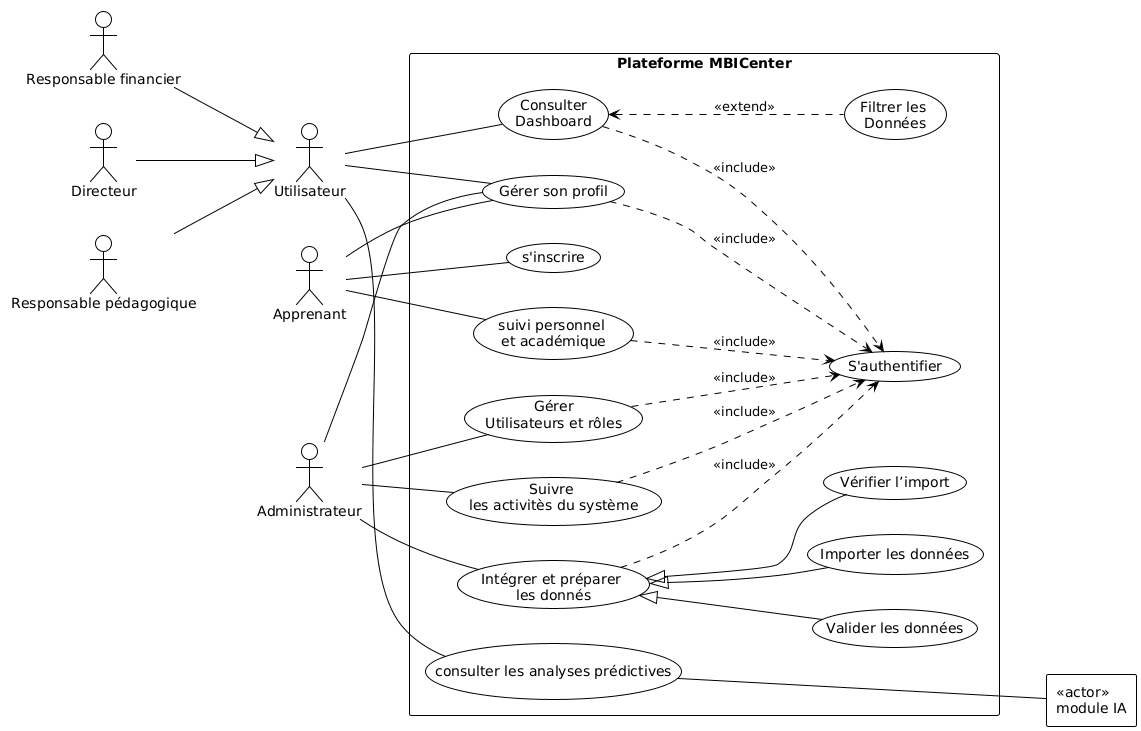
\includegraphics[scale=0.3]{project/images/XLNBRjD05Dr7oZzSkWb8f6fIAIeeYcgI097wW9PqWIf5KtkIZZGUcvbnH4MHsF89x5WshFa3_mbVmXaxiLCdRRE8VEyzz_sOGsEPjaaewODabayZ7VB9cz5av4twKHXBRdczzinUyv1JB9bGzLgz9ldKaer8YzcrfK1exbiHPQ863TB5L2ZX61HmGyotFD46tpHZYNyDUs15cdREk8aZPT.png}
  \caption{ Diagramme de cas d'utilisation globale}
  \label{fig:diagrammme de cas d'utilisation globale}
\end{figure}


\section{Pilotage du projet avec Scrum}
\label{cap:Pilotage du projet avec Scrum}
Dans le cadre de la gestion agile du projet, nous avons opté pour la méthodologie Scrum, qui permet une meilleure organisation des tâches et une priorisation progressive des besoins à travers un backlog produit structuré.

\subsection{Équipe et rôle}
Le bon déroulement et la réussite du projet dépendent d’une répartition efficace des rôles au sein de l’équipe, chacun apportant sa contribution spécifique

\begin{itemize}[label=\textbullet]
  \item \textbf{Product Owner}: Mme Taycir Chouk
  \item \textbf{Scrum Master}: Mme Leila Bayoudhi
  \item \textbf{Development Team }: Mme Mariem khlifi, Mme ferdaws maraach
\end{itemize}




\subsection{Le Backlog du produit}
Le Backlog produit regroupe l’ensemble des fonctionnalités de la plateforme sous forme de User Stories comme indiqué par le tableau \ref{tab:backlog_produit}. Chaque User Story décrit une fonctionnalité du point de vue de l’utilisateur final et est classée par priorité  selon la méthode MoSCoW, qui classe les éléments indispensables (Must), importantes (Should), optionnelles (Could) et non prévues pour cette version (Won’t), afin de réaliser d’abord les éléments les plus importants.
 
\small
\begin{longtable}{|p{1cm}|p{4cm}|p{10cm}|p{1.5cm}|}
\caption{Backlog produit}
\label{tab:backlog_produit} \\
\hline
\textbf{ID} & \textbf{Fonctionnalité} & \textbf{User Story} & \textbf{Priorité} \\
\hline
\endfirsthead
\hline
\textbf{ID} & \textbf{Fonctionnalité} & \textbf{User Story} & \textbf{Priorité} \\
\hline
\endhead

% --- US01 : Authentification ---
\multirow{3}{*}{\textbf{1}} & \multirow{3}{*}{\textbf{Authentification}}
& En tant qu'utilisateur, je veux m'authentifier de manière sécurisée pour accéder aux données selon mon rôle. & M \\
\cline{3-4}
& & En tant qu'apprenant, je veux pouvoir créer un compte sur la plateforme afin de m'inscrire à une formation. & M \\
\cline{3-4}
& & En tant qu'utilisateur, je veux pouvoir réinitialiser mon mot de passe oublié afin de retrouver l'accès à mon espace personnel en toute sécurité. & M \\
\hline

% --- US02 : Gestion des utilisateurs ---
\multirow{3}{*}{\textbf{2}} & \multirow{3}{*}{\textbf{Gestion des utilisateurs}}
& En tant qu'administrateur, je veux gérer les utilisateurs (activer, désactiver, modifier) et traiter les inscriptions. & M \\
\cline{3-4}
& & En tant qu'administrateur, je veux attribuer et gérer les rôles et permissions pour contrôler les accès. & M \\
\cline{3-4}
& & En tant qu'administrateur, je veux modifier et configurer les profils personnels des utilisateurs. & M \\
\hline

% --- US03 : Gestion des sessions de formation---
\multirow{4}{*}{\textbf{3}} & \multirow{4}{*}{\textbf{\shortstack[1]{Gestion des sessions \\ de formation}}}
& En tant que responsable pédagogique, je veux organiser et gérer les sessions de formation afin d'assurer le suivi et le bon déroulement des formations. & M \\
\hline

% --- US04 : Espace apprenant ---
\multirow{4}{*}{\textbf{4}} & \multirow{4}{*}{\textbf{Espace apprenant}}
& En tant qu'apprenant, je veux être redirigé automatiquement vers la page d'inscription lors de ma première connexion, afin de rejoindre une session avant d'accéder aux autres modules. & M\\
\cline{3-4}
& & En tant qu'apprenant, je veux voir un résumé de mes statistiques (formations inscrites, sessions à venir, moyenne générale) afin d'avoir une vue d'ensemble de mon parcours. & S\\
\cline{3-4}
& & En tant qu'apprenant, je veux consulter la liste des formations auxquelles j'ai participé, afin de suivre mon avancement. & S\\
\cline {3-4}
& & En tant qu'apprenant, je veux consulter les formations disponibles auxquelles Je n’ai pas encore participé, afin de découvrir de nouvelles opportunités d'apprentissage. & S\\
\cline {3-4}
& &  En tant qu'apprenant, Je veux participer à une session disponible d’une formation, afin de rejoindre une promotion active. & M\\
\cline {3-4}
& &  En tant qu'apprenant, je veux annuler ma participation à une session, afin de me désinscrire si mes disponibilités changent. & S\\
\cline{3-4}
& & En tant qu'apprenant, je veux consulter l'historique de toutes mes inscriptions passées et actuelles, afin de garder une trace de mon parcours. & C\\
\cline{3-4}
&& En tant qu'apprenant, je veux consulter mon emploi du temps complet (filtrable par semaine ou par mois), afin d'organiser mon agenda. & S\\
\cline{3-4}
& & En tant qu'apprenant, je veux consulter la synthèse de toutes mes notes par formation, afin d'évaluer mes performances globales. & C\\
\cline{3-4}
&& En tant qu'apprenant, je veux consulter la liste paginée de tous mes paiements (filtrables par formation, session ou date), afin de suivre ma situation financière. & S\\
\cline{3-4}
&& En tant qu'apprenant, je veux attribuer une note et un commentaire à une formation que j'ai suivie, afin de partager mon retour d'expérience. & C \\
\hline
% --- US05 : Alimentation des données ---
\multirow{4}{*}{\textbf{5}} & \multirow{4}{*}{\textbf{Alimentation des données}}
& En tant qu'administrateur, je veux importer les données brutes (raw data) pour centraliser les informations. & M \\
\cline{3-4}
& & En tant qu'administrateur, je souhaite que le système détecte automatiquement les erreurs dans les données importées afin de garantir leur qualité. & M \\
\cline{3-4}
& & En tant qu'administrateur, je veux valider ou rejeter les données importées afin que seules les données correctes soient stockées dans la base de données. & M \\
\cline{3-4}
& & En tant qu'administrateur, je souhaite charger les données validées dans la base de données afin qu'elles puissent être utilisées pour l'analyse et la production de rapports. & S \\
\hline
% --- US06 : Visualisation et analyse des données --- 
\multirow{6}{*}{\textbf{6}} & \multirow{6}{*}{\textbf{\shortstack[l]{Visualisation et \\ analyse des données}}} & En tant qu’utilisateur interne, je veux analyser les données du centre afin de comprendre les performances des activités. & M \\
 \cline{3-4}
& & En tant qu’utilisateur interne, je veux visualiser les indicateurs de performance sous forme de graphiques afin de suivre l’évolution des résultats. & M \\
\cline{3-4} & & En tant qu’utilisateur interne, je veux consulter des tableaux de bord afin de suivre les KPIs du centre. & M \\
\cline{3-4} & & En tant qu’utilisateur interne, je veux filtrer les données afin d’affiner mes analyses selon différents critères. & S \\ 
\cline{3-4} & & En tant que utilisateur interne, je veux exporter des rapports afin de partager les analyses et les résultats du centre. & M \\
\cline{3-4} & & En tant qu'utilisateur interne, je veux recevoir des notifications et alertes afin d'être informé en temps réel de tout événement important lié au fonctionnement du centre. & S \\ 
\hline


% --- US07 : Module prédictif et recommandations ---
\multirow{4}{*}{\textbf{7}} & \multirow{4}{*}{\textbf{\shortstack[l]{Module prédictif \\ et recommandations}}}
& En tant que responsable pédagogique, je veux recevoir des alertes sur les risques d'abandon générées par l'IA afin d'intervenir rapidement auprès des apprenants en difficulté. & C \\
\cline{3-4}
& & En tant que responsable financier, je veux prévoir les revenus afin de planifier le budget. & C \\
\cline{3-4}
&& je veux pouvoir prédire la probabilité de survenue de sessions déficitaires afin d'anticiper les risques financiers pour optimiser la rentabilité de l'entreprise. & C\\
\cline{3-4}
& & En tant que directeur, je veux des capacités d'analyse prédictive (prévision des inscriptions) afin d'anticiper les besoins futurs. & C \\
\cline{3-4}
& & En tant que Directeur, je veux accéder à des recommandations stratégiques basées sur l'analyse des données, afin de mieux prioriser les actions, déléguer les responsabilités et améliorer les performances globales de l'établissement. & C \\
\hline
\end{longtable}

\subsection{Planification des sprints}
Après avoir finalisé et ordonné le backlog produit, nous avons procédé à une estimation précise
des durées prévisionnelles de chaque sprint. Suite à une évaluation détaillée de la charge de travail,
nous avons défini 3 versions principales.

\noindent Le tableau \ref{tab:release_planning} présente la répartition détaillée de notre planification des sprints, en soulignant:
\begin{itemize}

  \item  La durée estimée de chaque sprint.
  \item Les principales fonctionnalités à développer.
  \item Les objectifs spécifiques de chaque version
 \end{itemize}
\begin{table}[H]
\centering
\caption{Planification des sprints}
\label{tab:release_planning}
\begin{adjustbox}{width=\textwidth}
\begin{tabular}{|c|c|l|c|}
\hline
\textbf{Release ID} & \textbf{Sprint} & \textbf{Nom du Sprint} & \textbf{Estimation (jours)} \\
\hline

\multirow{2}{*}{Release 1} 
& 1 & Authentification & 10 \\
\cline{2-4}
& 2 & Gestion des utilisateurs & 10 \\
\hline

\multirow{3}{*}{Release 2} 
& 3 & Gestion des sessions de formation & 10 \\
\cline{2-4}
& 4 & Espace apprenant & 10 \\
\cline{2-4}
& 5 & Alimentation des données & 10 \\
\hline

\multirow{2}{*}{Release 3} 
& 6 & Visualisation et analyse des données & 10 \\
\cline{2-4}
& 7 & Module prédictif et recommandations & 10 \\
\hline

\end{tabular}
\end{adjustbox}
\end{table}

\section{Conclusion} 


Ce chapitre nous a permis de définir précisément "pour qui" et "comment" nous allons construire cette solution. En comprenant les besoins des utilisateurs et en structurant notre méthode de travail agile, nous avons désormais une vision claire du projet. Forts de ces bases solides, nous pouvons maintenant aborder, dans le chapitre suivant, le choix des technologies et la conception technique qui permettront de transformer ces besoins en une plateforme réelle.